\section{Lussekatter}
Nok til to brett med svære lussekatter
\subsection{Norsk}

\paragraph{Ingredienser}
\begin{itemize}[noitemsep]
	\item 50 gram TINE Ekte Meierismør
	\item 5 dl TineMelk Hel
	\item 50 gram gjær
	\item 1 gram safran
	\item 150 gram sukker
	\item $\frac{1}{2}$ ts salt
	\item 2 ts kardemomme
	\item 700 gram speltmel
	\item Pensling og pynt: 1 egg og 1 dl rosiner
\end{itemize}

\paragraph{Framgangsmåte}
\begin{enumerate}[noitemsep]
	\item Smelt smøret og tilsett melken. Smuldre gjæren oppi pannen med melk og smør
	\item Hvis safranen ikke er finmalt må den knuses i en mortar eller kuttes fint opp. Ellers blir ikke det skikkelig gult og du vil få røde flekker på baksten
	\item Bland sukker, mel, salt og kardemomme i en bakebokk. Bland og tilsett væslen
	\item La deigen heve under plast på et lunt sted til dobbel størrelse
	\item Sett stekeovnen på 200 \degree C
	\item Strø litt mel på bordet og elt deigen godt
	\item Del deigen i biter og trill dem til lange fingertykke pølser og del i ca. 32 biter ( 16*2 brett, 4x4 lussekatter på brettet)
	\item Form lussekattene som på Tines godkjente lussekattfigurmal, figur  \ref{lussekatter}
	\item Legg de ferdig formede lussekattene på stekeplaten og la dem heve under plast på et lunt sted i ca. 15 minutter
	\item Pensle med sammenvispet egg og pynt med rosiner
	\item Stek lussekattene på 200 grader i  ca 10 minutter
	\item La de avkjøles litt på rist før servering. De smaker aller best litt lunkne
\end{enumerate}

Tips: Halvparten av denne mengden er nok til Vibecke og Fredrik, basert på baksten 2016.

Kilde: Orginalt fra \href{http://www.tine.no/oppskrifter/bakst/sot-gjarbakst/lussekatter}{Tine.no}, kraftig modifisert


\subsection{Français}
\paragraph{Ingrédients}
\begin{itemize}[noitemsep]
	\item 50g de beurre
	\item 5 décilitre de lait entier
	\item 50g de levure
	\item 1g de safran
	\item 150g de sucre
	\item 1/2 cuillére à café de sel
	\item 2 cuillére à café de cardamome
	\item 13 décilitre de farine
	\item 1 eouf
	\item 1 décilitre de raisins secs
\end{itemize}

\paragraph{Préparition}
\begin{enumerate}[noitemsep]
	\item Fait fondre le beurre. Ajouter le lait. Émiette la levure dans un bol et ajouter le lait et le beurre
	\item Écraser le safran dans un mortier et l'ajouter  dans le bol
	\item Ajouter le sucre, le sel, la cardamome, le safran et la farine jusqu'à ce que pâte soit ferme
	\item Laisser lever la pâte jusqu'à c'est doublé de taille.
	\item Pétrir la pâte et faire des saucisses de l'epaisseur d'un doigt. Divisé en 30 morceaux
	\item Façonner la pâte dans les formes vous voulez, laissez-les reposes pendant 15 minutes et bedigeonner avec l'oeuf et décorer avec des raisins secs
	\item Faire cuire dans le four á 250 degrés pour 5--8 minutes.
	\item Refroidir sur une grille
	\item Voila
\end{enumerate}


\href{https://fr.wikipedia.org/wiki/Lussekatt}{fr.wikipedia/lussekatt}


\begin{figure}[p]
	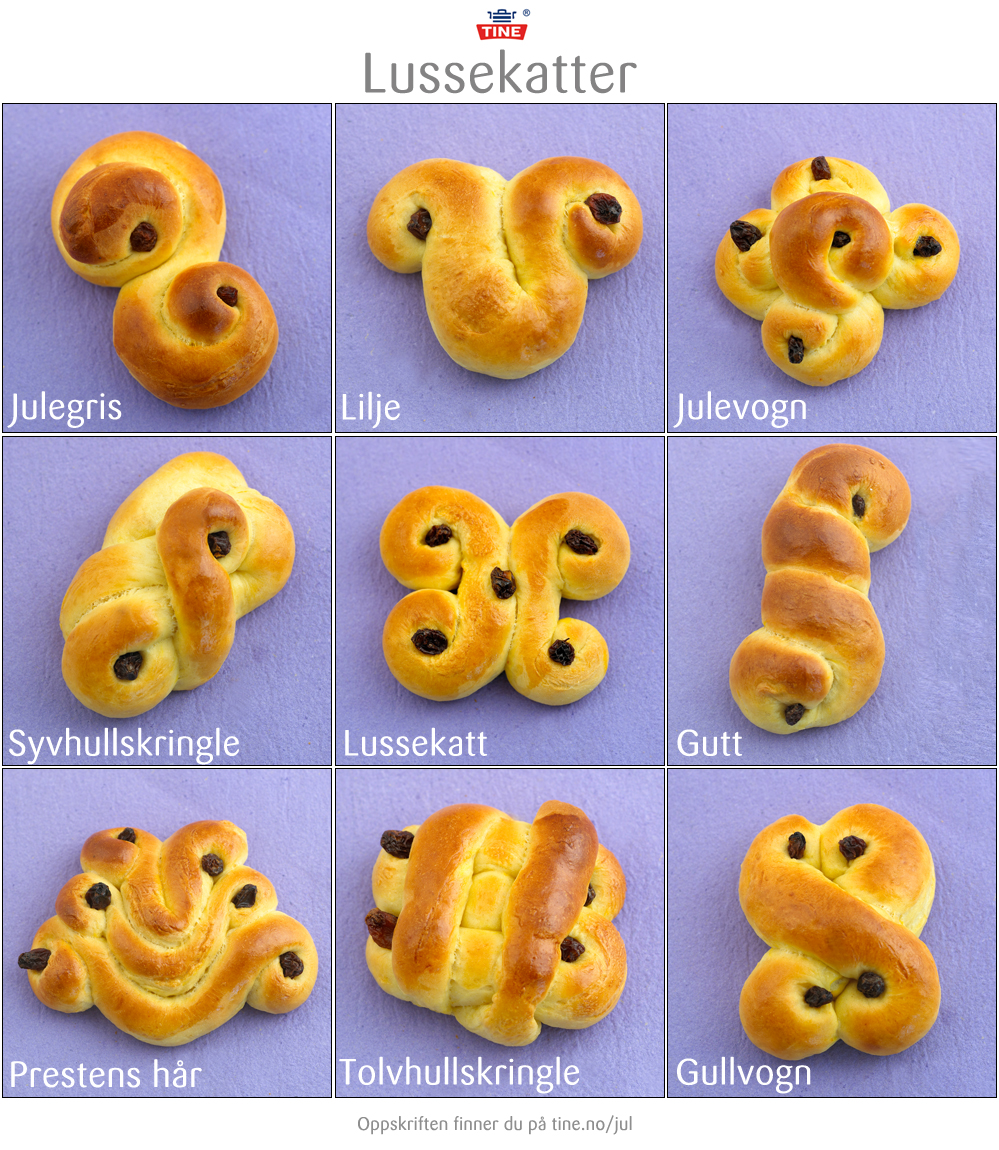
\includegraphics[width=\textwidth]{bilder/lussekatter.png}
	\caption[Lussekatter]{Lussekatter. Kilde \href{http://www.tine.no/imageresize/383493_999_1150.png}{Tine.no}}
	\label{lussekatter}
\end{figure}
